%---Packages---%
\documentclass[a4paper,11pt]{article}
\usepackage[left=2.5cm,top=2cm,right=2cm,nohead]{geometry}
\usepackage[french]{babel}
\usepackage[T1]{fontenc}
\usepackage[utf8]{inputenc} 
\usepackage{graphicx}
\usepackage{float}
\usepackage{amsmath}
\usepackage{amsfonts}
\usepackage{amssymb}
\usepackage{listings}
\usepackage{mdwlist}
\usepackage[usenames,dvipsnames]{color}
\usepackage[stable]{footmisc}%To include footnotes in 'section' parts
\usepackage{hyperref}
\usepackage{setspace}
\usepackage{eurosym}
\usepackage[section]{algorithm} % [section] is use to define the numbering mode
\usepackage{algorithmic} 
\usepackage{verbatim}
\lstloadlanguages{R}

%---Insertion de code---%
\definecolor{lightgray}{gray}{0.95}

\lstset
{           
backgroundcolor=\color{lightgray},
keywordstyle=\color{Red}\bfseries,
ndkeywordstyle=\color{darkgray}\bfseries,
commentstyle=\color{Green},
stringstyle=\color{Orange},
basicstyle=\scriptsize,       % the size of the fonts that are used for the code
numbers=left,                   % where to put the line-numbers
numberstyle=\tiny,      % the size of the fonts that are used for the line-numbers
stepnumber=2,                   % the step between two line-numbers. If it's 1 each line will be numbered 
numbersep=5pt,                  % how far the line-numbers are from the code
showspaces=false,               % show spaces adding particular underscores
showstringspaces=false,         % underline spaces within strings
showtabs=false,                 % show tabs within strings adding particular underscores
tabsize=2,	                    % sets default tabsize to 2 spaces
captionpos=b,                   % sets the caption-position to bottom
breaklines=true,                % sets automatic line breaking
breakatwhitespace=false,        % sets if automatic breaks should only happen at whitespace
%title=\lstname,                 % show the filename of files included with \lstinputlisting & 
escapeinside={\%*}{*)},         % if you want to add a comment within your code
morekeywords={*,...}            % if you want to add more keywords to the set
extendedchars=true
}

%---Liens---%
\hypersetup{
unicode=false,          % non-Latin characters in Acrobat’s bookmarks
pdftoolbar=true,        % show Acrobat’s toolbar?
pdfmenubar=true,        % show Acrobat’s menu?
pdffitwindow=false,     % window fit to page when opened
pdfstartview={FitH},    % fits the width of the page to the window
pdftitle={PPH - Comment manager une équipe de bénévoles associatifs ?},    % title
pdfauthor={Balthazar Rouberol},     % author
pdfsubject={PPH - Comment manager une équipe de bénévoles associatifs ?},   % subject of the document
pdfcreator={Balthazar Rouberol},   % creator of the document
pdfkeywords={PPH, management, travail d'équipe, bénévolat}, % list of keywords
pdfnewwindow=true,      % links in new window
colorlinks=true,       % false: boxed links; true: colored links
linkcolor=black,          % color of internal links
citecolor=black,        % color of links to bibliography
filecolor=white,      % color of file links
urlcolor= NavyBlue,           % color of external links
bookmarks=true,% show bookmarks bar?
bookmarksopen=false,
bookmarksnumbered = false      
}%

%%---Page de garde---%
\makeatletter
\def\clap#1{\hbox to 0pt{\hss #1\hss}}%
\def\ligne#1{%
\hbox to \hsize{%
\vbox{\centering #1}}}%
\def\haut#1#2#3{%
\hbox to \hsize{%
\rlap{\vtop{\raggedright #1}}%
\hss
\clap{\vtop{\centering #2}}%
\hss
\llap{\vtop{\raggedleft #3}}}}%
\def\bas#1#2#3{%
\hbox to \hsize{%
\rlap{\vbox{\raggedright #1}}%
\hss
\clap{\vbox{\centering #2}}%
\hss
\llap{\vbox{\raggedleft #3}}}}%
\def\maketitle{%
\thispagestyle{empty}\vbox to \vsize{%
\haut{}{\Large \@blurb}{}
\vfill
\vspace{1cm}
\begin{flushleft}

\huge \@title
\end{flushleft}
\par
\hrule height 4pt
\par

\begin{flushright}
\Large \@author
\par
\end{flushright}
\vspace{1cm}
\vfill
\vfill
\bas{}{INSA Lyon - 4BIM\\[0.15cm] \today}{}
}%
\cleardoublepage
}
%\def\date#1{\def\@date{#1}}
\def\author#1{\def\@author{#1}}
\def\title#1{\def\@title{#1}}
\def\location#1{\def\@location{#1}}
\def\blurb#1{\def\@blurb{#1}}
\date{\today}
\makeatother
\title{\textbf{PPH - Comment \og manager \fg{} une équipe de bénévoles associatifs ?}}
\author{par Balthazar Rouberol}
\location{Lyon}
\blurb{%
\begin{center}
	\mbox{\textbf{Projet Personnel en Humanités}}
	\\
	\mbox{\normalsize Tuteur : Joachim Revez}
	\\[3.5cm]
	%\includegraphics[scale = 1]{./Net.jpg}\\[2cm]
\end{center}
\setlength\fboxsep{0pt}
\setlength\fboxrule{1pt}
}% p


\begin{document}
\maketitle
\newpage

\section{Introduction}
Durant ma 4$^e$ année à l'INSA de Lyon, je me suis engagé au Bureau des Élèves (BdE), l'une des plus grosses associations du campus, en tant que vice-président responsable de la vie associative. Mon rôle était d'assurer une forte cohésion au sein de la communauté associative, d'organiser des formations pour les nouveaux bureaux, de pouvoir répondre à leur questions quotdiennes, etc. Au cours de l'année, j'ai donc interagi de façon soutenue avec une grande majorité des 125 associations qui font la force et la diversité de ce campus. En plus de ce rôle de vecteur d'information, j'ai mis un point d'honneur à aider ces associations lors de leurs manifestations, si celles-ci avaient besoin d'organisateurs \og softs \fg{}. \\

Tout cela m'a donc offert l'opportunité de pouvoir observer leur fonctionnement, et leur manière, chaque fois unique et réinventée, de travailler en équipe et d'assurer une bonne cohésion au sein de l'association.\\

Le but de ce PPH est donc de s'interroger sur les façons pour un membre de bureau ou un chef d'équipe de \og manager \fg{} les bénévoles dont il est responsable, afin d'instaurer une atmosphère agréable et productive. Pour cela, nous allons analyser comment des équipes associatives sont gérées à l'INSA, établir un parallèle entre le management associatif et le management en entreprise pour en percevoir les différences. Forts de ces réflexions, nous tenterons de comprendre comment instaurer une dynamique de travail de groupe sur le long terme dans une association.

\section{La gestion d'équipe - deux cas d'étude : Indication et le BdE}
Lors de ma scolarité à l'INSA, je me suis investi au bureau de deux associations : à Indiaction, en temps que secrétaire, et au BdE, en temps que reponsable de la vie associative. Ces deux expériences au sein d'associations radicalement différentes vont nous servir de bases de réflexion.\

\subsection{La gestion de l'équipe d'Indiaction}
Indiaction est une association humanitaire d'une quinzaine de personnes, oeuvrant à l'amélioration des conditions de vie dans un orphelinat situé au nord de l'Inde, ainsi qu'à l'apport d'eau potable dans un village du Penjab. L'association est visible à la Fête des Lumières, à Noël, à l'occasion d'une vente d'artisanat et de produits indiens, lors de la semaine asiatique et surtout lors de la semaine indienne. La vie de l'association est donc rythmée par ces événements, qui demandent un degré d'investissement différent : la majorité des efforts sont concentrés sur la semaine indienne.\\

Il est demandé aux membres actifs une présence à la réunion hebdomadaire, de l'investissement sur les différentes manifestations, ainsi qu'être force de proposition lors de la planification de ces événements. Chaque membre actif s'investit là ou sa compétence est la plus appréciée  : composition d'affiches, préparation de plats, etc. Les membres du bureau s'investissent au même titre que les membres actifs, en plus des responsabilités conférées par leur poste. Il n'est donc pas rare de voir le président à la vente d'artisanat, le secrétaire à l'élaboration d'une affiche, ou le trésorier faisant les courses.\\

La cohésion de l'équipe au sein de l'année passe par une ambiance \og bon enfant \fg{}{} lors les réunions, des sorties organisées dans des restaurants indiens, des soirées à la K-Fêt, etc. Les membres les plus motivés participent chaque années à un voyage en Inde, afin de se rendre à l'orphelinat et de participer aux travaux.\\

La petite structure de l'association implique une forte liberté d'engagement : il ya peu de flux d'argent au cours de l'année, ce qui permet au bureau de s'investir au quotidien et de ne pas s'\og engluer \fg{} dans la gestion administrative. Chaque membre actif peut facilement être en charge d'une tâche précise : commander des T-shirts, choisir et inviter des artistes, concevoir une affiche\ldots Son travail sera ensuite présenté au reste de l'équipe pour être critiqué, commenté puis validé. Le travail en équipe est bien sûr encouragé dans toutes les tâches créatives, ou contraignantes (compter les stocks, compter les caisses, \ldots) afin d'assurer une forte émulation dans l'équipe.

\subsection{La gestion d'équipe au Bureau des Élèves}
Le Bureau des Élèves a une strucure radicalement différente de celle d'Indiaction. Le premier élément frappant est son nombre de membres actifs : environ 230 cette année. Ceux-ci sont répartis dans une vingtaine d'équipes, regroupant des équipes de gestion, d'événementiel,de service, d'animation, etc : Bureau, Conseil d'Administration, CoWEI (organisateur du weekend d'intégration), Raid, Gala, High Five, DIPC (organisation du weekend de \og désintégration \fg{} des 2$^e$ années), Comité d'animation, animation interne, vie associative, services, Orga'If, communication, relations extérieures, Melt'INSA (accueil des élèves étrangers), Comité de Parrainage (acceuil des primos rentrants), Sponsoring, INSA Shop (vente de la ligne textile INSA) et développement durable. %VERIFIER SI EQUIPE MANQUANTE !
\\

Chacune de ces équipes est gérée par un responsable d'équipe et suivie par le vice-président chargé des équipes.
Ce double suivi est essentiel au bon fonctionnement de l'équipe et à sa bonne intégration dans l'association et sa politique. Le responsable de l'équipe assure sa gestion quotidienne, établit et suit le calendrier et délais à respecter, anime les réunions, présente les budgets au Conseil d'aministration\ldots Quant à lui, le VP-équipes assiste aux réunions en tant que représentant du bureau, afin d'être consulté en cas de problème, de question importante. Il apporte son expérience de la manifestation aux organisate\\
urs, et peut déconseiller, voire interdire, certaines prises de positions (propos déplacés dans le poly de parrainage, dans la vidéo d'intégration, etc). Il assure donc le lien entre l'équipe et le bureau, voire directement entre les équipes.\\

Depuis cette année, l'organisation des équipes a été repensé afin de ne pas écraser le VP-équipes sous le travail. Ce travail de liaison entre le bureau et l'équipe sera aussi assuré par d'autres membres du bureau, comme le montre l'organigramme ci dessous : 
\begin{figure}[h!]
	\centering
	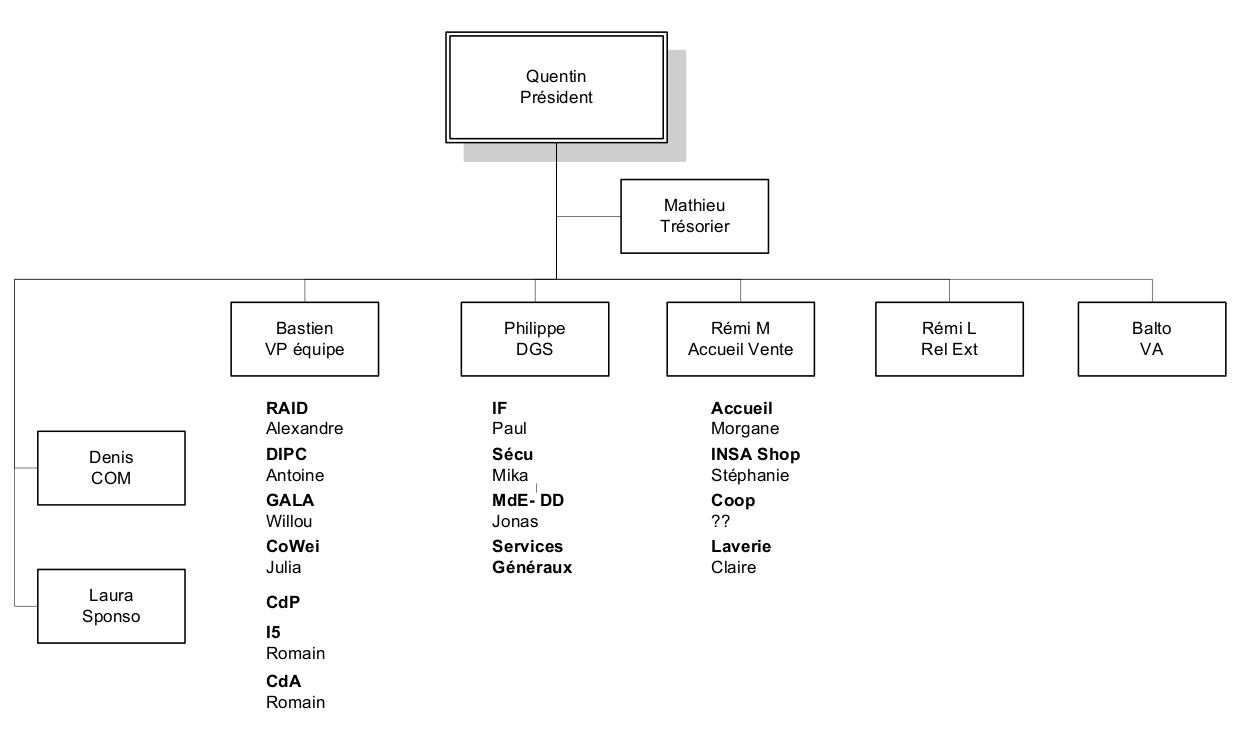
\includegraphics[scale=0.33]{IMG/organigramme.png}
	\caption{Organigramme des équipes et responsables d'équipes du BdE}
\end{figure}

L'animation interne de l'équipe est laissée à la charge du responsable, qui l'organisera comme bon lui semble.
Une animation destinée à tous les membres actifs est assurée en parallèle par l'équipe d'animation interne. Ainsi, c'est jusqu'à 200 personnes qui peuvent se retrouver lors de soirées raclette, de weekends ski, de soirées patinoires, de sorties acrobranches, ou même s'échanger des cadeaux à Noël.

\section{Différences entre management en entreprise et en association} 
\subsection{Définitions}
Avant de tenter d'établir les différences entre le management en entreprise et en association, attardons nous sur la définition m\^{e}me du management.\\

\mbox{
	\begin{minipage}{0.96\linewidth}
		\textbf{Management} (\href{http://fr.wikipedia.org/wiki/Management}{Définition Wikipedia}) : Le management ou la gestion est l'ensemble des techniques d'organisation de ressources qui sont mises en œuvre pour l'administration d'une entité, dont l'art de diriger des hommes, afin d'obtenir une performance satisfaisante. Dans un souci d'optimisation, il tend à respecter les intérêts et représentations des parties prenantes. \\
	\end{minipage}
}

La notion centrale est ici celle de performance. Celle-ci est bien sur centrale en entreprise, dont le but premier est le bénéfice, mais est plus difficile à appréhender dans le milieu associatif. En effet, les associations du campus sont toutes des associations de type loi de 1901. Leurs activités sont donc statutairement définies comme non lucratives.\\

\mbox{
	\begin{minipage}{0.96\linewidth}
		\textbf{Activité non lucrative} (\href{http://fr.wikipedia.org/wiki/Association\_\%C3\%A0\_but\_non\_lucratif}{Définition Wikipedia}) : Par activité non lucrative, on entend qu'elle peut faire payer des biens ou des services, mais le prix doit correspondre à un défraiement des dépenses nécessaires à ses activités et non pas à une activité commerciale ou productive. De fait, son objet ne doit pas être le même que les entreprises de négoce, de finance, d'assurance, etc, mais le plus souvent des activités culturelles, éducatives, religieuses, artistiques, sportives, familiales etc. \\ 
	\end{minipage}
}

On touche donc ici à une différence fondamentale entre le milieu associatif et l'entreprise. Dans une association,
la notion de \og performance \fg{} doit être largement adaptée.\\

\subsection{Notion de performance \og à l'insalienne \fg}
À l'INSA, la majorité des associations concillient une activité routinière et l'organisation d'une \og manifestation \fg{} (les 24h de l'INSA, le Forum Rhônes-Alpes, la nuit du volley, festival de bédéologie, semaine asiatique, semaine du développement durable, \ldots). Ces manifestations constituent le coeur des revenus financiers de ces associations et impliquent souvent une organisation conséquente, voire très importante, et nécessitent une forte implication de membres bénévoles. Toute tentative de définir la notion de performance d'une association doit donc concillier l'épanouissement des membres actifs dans les activités de l'association, la qualité des manifestations organisées et la bonne gestion financière.\\

Certaines associations, comme le BdE et l'ARGIL, peuvent être comparées à des petites entreprises, car elles proposent un service quotidien aux insaliens. \\En effet, le BdE leur propose l'achat de jetons de laverie, de tickets TCL, de vêtements, de nourriture, de fournitures scolaires, la disposition d'un parc de photocopieuses\ldots  et l'ARGIL propose un service de vente de boissons alcoolisées et non-alcoolisées. Leur résultat financier annuel (particulièrement pour l'ARGIL) dépend donc moins de manifestations que de leur ventes au quotidien. La notion de performance se rapproche donc de celle d'une entreprise, mais en aucun cas les critères d'épanouissement des membres actifs et de qualité de manifestation ne doivent être remis en cause.

\newpage


\end{document}